\documentclass[11pt]{article}
\usepackage[margin=1in]{geometry}
\usepackage[T1]{fontenc}
\usepackage{lmodern}
\usepackage{microtype}
\usepackage{booktabs}
\usepackage{graphicx}
\usepackage[round]{natbib}
\usepackage[hidelinks]{hyperref}
\setlength{\parskip}{4pt}
\setlength{\parindent}{0pt}

\title{\vspace{-1.5em}Do the Frey--Osborne Automation Scores Depend on Their Hand Labels?}
\author{Nyx(ius) Labs}
\date{Extended abstract, AI for Social Science Research Methods, Yale University, April 2027}

\begin{document}
\maketitle
\vspace{-1.5em}

\begin{abstract}
\noindent Social scientists often measure concepts with a classifier trained on a small set of hand
labels. A widely used example is the set of automation scores that Frey and Osborne computed for 702 US
occupations from 70 occupations they labeled by hand. The scores support the estimate that 47\% of US
employment is at high risk of automation. We refit their classifier from public files and changed the
labels, the classifier and the input data. Changing a single label moves the high-risk share between
37\% and 50\%. Across 200 simulated experts drawn from a later survey, the share follows how many of the 70
occupations the expert calls automatable; at the experts' average of 29 to 31, it is about 27\%. For about half of employment, whether an occupation falls above the cutoff depends on the
labels. The ordering of occupations is steadier: in 846 of 848 refits, occupations with higher scores lost
employment between 2012 and 2023.
\end{abstract}

\section{Introduction}
Many measures in the social sciences come from a classifier trained on a few dozen or a few hundred
cases that researchers labeled by hand. The labels are judgments. Authors report how well the classifier
recovers labels it did not see, but rarely how much the measure would change if the judgments had been
different.

\citet{frey2017} offer a clear case. With a group of machine-learning researchers, they labeled 70
occupations as automatable or not, trained a Gaussian-process classifier on nine O*NET variables, and
scored all 702 detailed occupations. Occupations with a probability of 0.7 or more held 47\% of US
employment. The scores are used as regressors in studies of health \citep{patel2018}, local labor
markets \citep{frank2018} and wages \citep{fossen2022}. To check the labels, Frey and Osborne trained
the classifier on half of them and predicted the other half. The fit was good, and they concluded that
``slight modifications to this set are unlikely to lead to substantially different results.'' We test
that sentence.

Earlier work changed other parts of the design. \citet{arntz2016} and \citet{nedelkoska2018} moved from
occupations to individual jobs. \citet{lorenz2023} collected new labels in Austria and compared model
families. \citet{coelli2019} asked whether the published scores predict employment change. Corrections for regressions on machine-learned variables \citep{wang2020, fong2021, battaglia2024}
need a sample of correctly labeled cases. None exists here, because the labels are forecasts.

Section~3 reports three results in turn: (1) the share of employment at high risk depends on a few
labels, and mostly on how many are marked automatable; (2) for about half of employment, an occupation's side of the 0.7 cutoff depends on the labels;
(3) the ordering of occupations holds, and it predicts later employment change.

\section{Data and methods}
\textbf{Data.} All inputs are public. The appendix of \citet{frey2013} lists each occupation's
probability and the 70 hand labels (37 automatable). The nine input variables come from O*NET 17.0
(July 2012), the first release coded to the 2010 occupation codes. Employment by occupation comes from
the American Community Survey (ACS) for 2012, 2019 and 2023; we follow 406 occupation groups across the
2018 revision of the codes.

\textbf{Refit.} We fit a Gaussian-process classifier with a squared-exponential kernel and one length
scale per variable \citep{rasmussen2006}. We use scikit-learn's Laplace approximation rather than the
expectation propagation of the original code. Our probabilities correlate with the published ones at
0.99, and 98\% of occupations fall on the same side of 0.7. With 2012 ACS employment, the published
scores put 44.5\% of employment at high risk, close to the 47\% the authors found with 2010 BLS data.

\textbf{Changes.} We refit the classifier under four kinds of change:
\begin{itemize}\setlength{\itemsep}{0pt}
\item \emph{One label:} each of the 70 labels reversed in turn.
\item \emph{Several labels:} 7 labels (10\%) reversed at random, 100 times; or a random 60 of the 70
used for training, 200 times.
\item \emph{Labels toward expert opinion:} \citet{walsh2018} asked about 300 AI and robotics experts to
label the same 70 occupations; on average they marked 29 to 31 as automatable (standard deviation 10),
against 37. He reports these counts, not each expert's labels. We switch 7 random ``automatable'' labels
to ``not'', 100 times. We also simulate 200 single experts: each draws a count from Walsh's reported
distributions, and we make the fewest label changes that reach it.
\item \emph{Classifier and data:} six other classifiers, and O*NET 28.0 (2023) in place of 17.0.
\end{itemize}

\textbf{Measures.} For each refit we compute the share of 2012 employment with probability 0.7 or more,
and regress log employment change from 2012 to 2023 on the probability across the 406 groups, weighted
by employment. For each occupation we ask whether its 90\% interval across refits contains 0.7.

\section{Results}
\subsection{The high-risk share depends on a few labels}
Figure~\ref{fig:main} (left) shows the high-risk share in each refit. Reversing one label moves it
between 37\% and 50\%. Reversing 7 at random moves it between 28\% and 49\% (middle 90\% of refits).
The six other classifiers
predict held-out labels about as well as the original (area under the curve 0.85 to 0.91), yet give
shares from 37\% to 51\%.

The cause is how the labels were chosen. Frey and Osborne labeled the occupations they were most sure
of. Many large occupations lie between labeled occupations of opposite kinds, so one changed label can
move the classifier's boundary across them. For example, relabeling claims adjusters as not automatable
lowers the score of retail salespersons, the largest occupation, from 0.92 to 0.38. Predicting held-out
labels measures agreement only among the labeled occupations, so it cannot reveal this.

For the simulated experts, the share depends mostly on how many occupations each marks automatable.
Figure~\ref{fig:count} plots the two; the rank correlation is 0.97. An expert at the survey average of
29 to 31 gives a median share of 27\%, and one who marks 25 or fewer usually gives under 5\%. Fewer
``automatable'' labels should give fewer high-risk jobs; the point is the size. Removing a fifth of the
``automatable'' labels removes about two fifths of the high-risk share, so the 47\% figure largely
reflects how often the labelers said ``automatable''.

\begin{figure}[h]
\centering
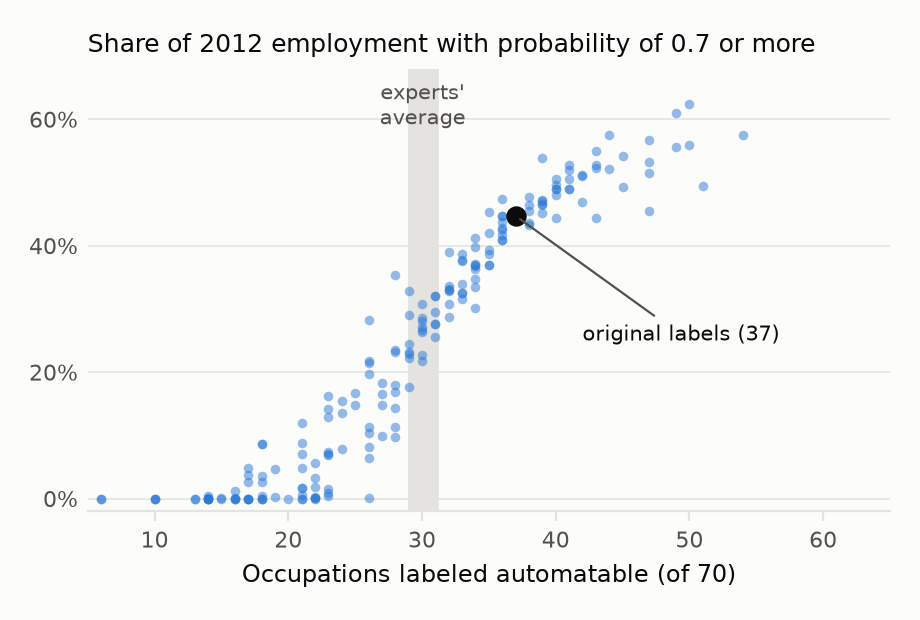
\includegraphics[width=0.5\textwidth]{figure2.png}
\caption{High-risk share against the number of occupations labeled automatable, for 200 simulated
experts. The gray band is the average in \citet{walsh2018}.}
\label{fig:count}
\end{figure}

\subsection{Half of employment is near the cutoff}
The same instability holds for single occupations. When 7 random labels change, 53\% of 2012
employment is in occupations whose 90\% interval contains 0.7. Even when only 10 of the 70 labels are
left out, the figure is 32\%. Table~\ref{tab:occ} shows the ten largest occupations. For six of them,
one changed label is enough to move the score across 0.7.

\begin{table}[h]
\centering\small
\begin{tabular}{lcccc}
\toprule
 & Employment & Published & One label & 7 labels changed \\
Occupation & 2012 (m) & score & changed (range) & (middle 90\%) \\
\midrule
Retail salespersons                     & 3.5 & 0.92 & 0.38--0.94 & 0.38--0.87 \\
Supervisors of retail sales workers     & 3.0 & 0.28 & 0.02--0.44 & 0.05--0.47 \\
Customer service representatives        & 2.5 & 0.55 & 0.35--0.84 & 0.24--0.76 \\
Waiters and waitresses                  & 2.2 & 0.94 & 0.71--0.96 & 0.67--0.90 \\
Accountants and auditors                & 2.1 & 0.94 & 0.83--0.95 & 0.64--0.92 \\
Laborers and freight movers, hand       & 2.0 & 0.85 & 0.61--0.91 & 0.50--0.88 \\
Construction laborers                   & 1.6 & 0.88 & 0.50--0.96 & 0.47--0.89 \\
Stock clerks and order fillers          & 1.6 & 0.64 & 0.30--0.91 & 0.36--0.89 \\
Maids and housekeeping cleaners         & 1.5 & 0.69 & 0.45--0.92 & 0.46--0.85 \\
Postsecondary teachers                  & 1.4 & 0.03 & 0.03--0.15 & 0.07--0.37 \\
\bottomrule
\end{tabular}
\caption{Scores of the ten largest occupations under changes to the hand labels. Employment from the
2012 ACS.}
\label{tab:occ}
\end{table}

\subsection{The ordering holds and predicts employment change}
Although the level of each score moves, the order of occupations changes less: the other classifiers
have a rank correlation of 0.82 to 0.88 with the original. Figure~\ref{fig:main}
(right) relates the scores to what happened next. With the published scores, an occupation scored 1
grew about 23 log points less from 2012 to 2023 than one scored 0 (standard error 0.07). The slope is
negative in 846 of 848 refits, though its size ranges from $-0.12$ to $-0.39$ (middle 90\%) when 7 labels change. This
check agrees with \citet{coelli2019} in one respect: once we control for a routine-task index
\citep{acemoglu2011}, the slope stays negative in 98\% of refits but is more than two standard errors
below zero in only 57\%. Much of what the scores order is routine work.

\begin{figure}[h]
\centering
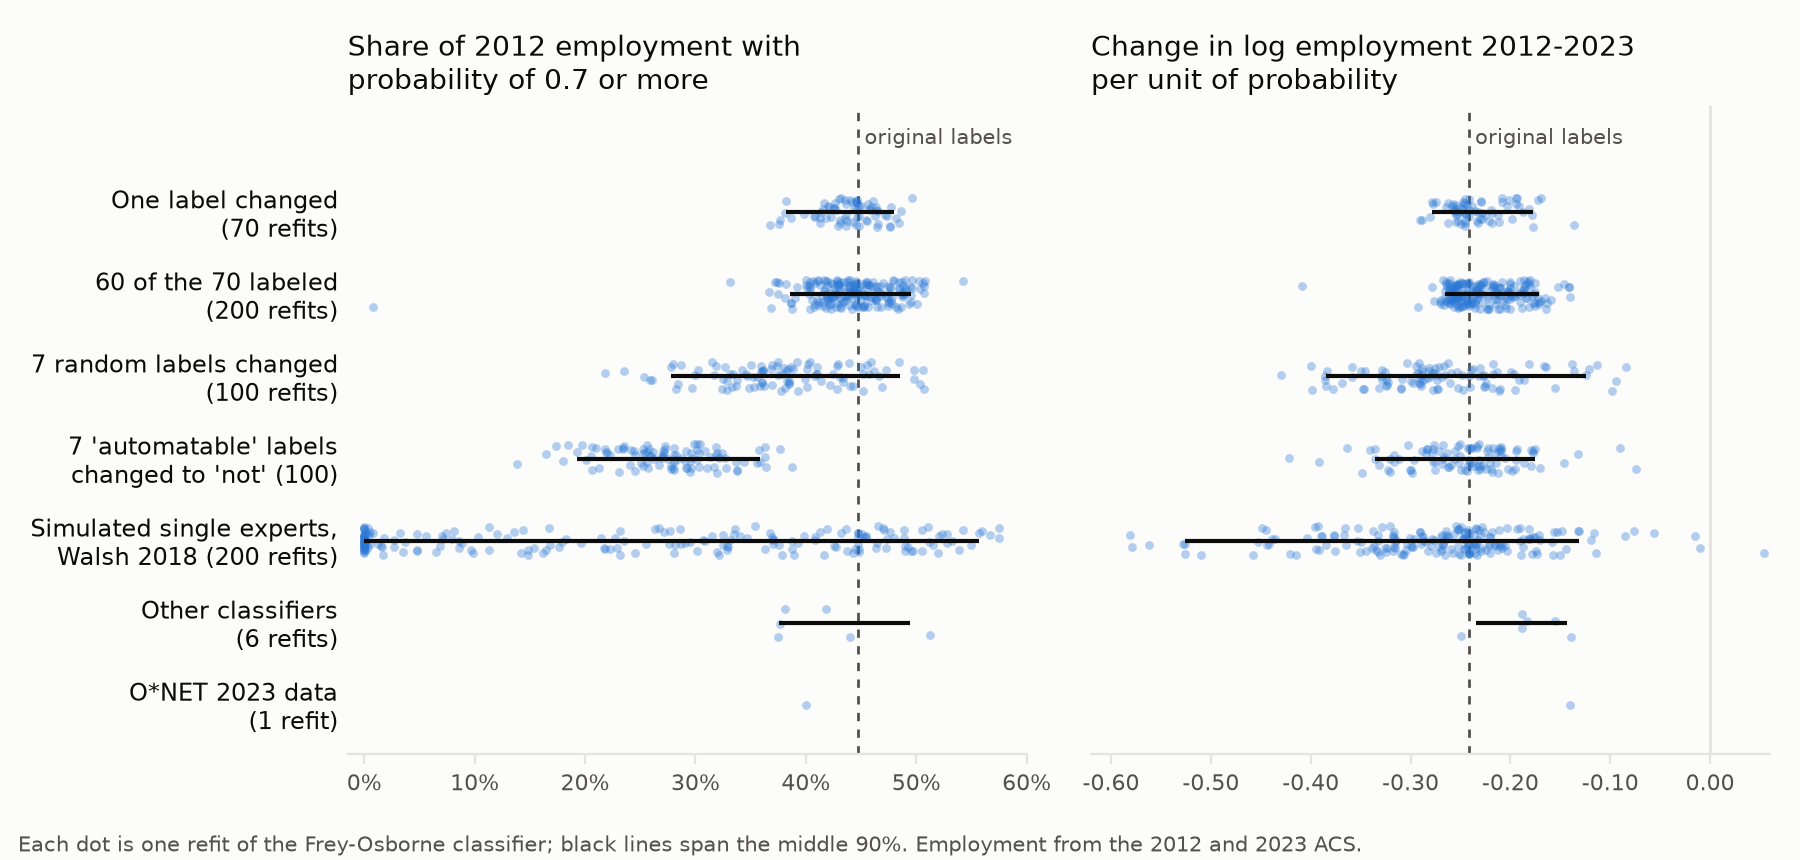
\includegraphics[width=0.84\textwidth]{figure1.png}
\caption{Share of employment at high risk (left) and slope of employment change on the score (right),
by kind of change. Each dot is one refit.}
\label{fig:main}
\end{figure}

\section{Checks and limits}
\textbf{Employment data.} Where one ACS code covers several occupations, we split its employment
equally among them. The published scores give a similar share with ACS and BLS data (44.5\% and 47\%).

\textbf{Simulated labels.} Walsh did not publish each expert's labels, so we choose at random which
labels change. Because we make only the fewest changes that reach each count, two experts with the
same count as Frey and Osborne count as agreeing; actual disagreement is larger. We plan to collect a
second set of labels from independent coders.

\textbf{Time horizon.} Frey and Osborne expected change over ``a decade or two''; we use later
employment only to check the ordering. Ending the window in 2019 gives a smaller slope, negative in 843 of
848 refits.

\section{Conclusion}
A classifier trained on a few hand labels turns a small number of judgments into a measure for every
case. For the Frey--Osborne scores, the 47\% figure largely reflects how many occupations the labelers
called automatable, and the class of many large occupations depends on single labels; the ordering of occupations depends on them much less. Users can treat such scores as a ranking rather than as counts above a cutoff. Agreement on held-out labels does not show that a measure is stable. Before the workshop
we will add a second, independent set of labels and apply the same checks to other measures built from
hand labels. Code and the refit scores for every occupation: \url{https://github.com/brandonyee-cs/autoscores}.

\textit{Requested format: lightning talk or talk; poster acceptable.}

\begingroup\footnotesize
\begin{thebibliography}{20}\setlength{\itemsep}{0pt}
\bibitem[Acemoglu \& Autor(2011)]{acemoglu2011} Acemoglu, D., \& Autor, D. (2011). Skills, tasks and
  technologies: Implications for employment and earnings. In \emph{Handbook of Labor Economics}, Vol.\ 4B,
  1043--1171. Elsevier.
\bibitem[Arntz et~al.(2016)]{arntz2016} Arntz, M., Gregory, T., \& Zierahn, U. (2016). The risk of
  automation for jobs in OECD countries: A comparative analysis. OECD Social, Employment and Migration
  Working Papers No.\ 189.
\bibitem[Battaglia et~al.(2024)]{battaglia2024} Battaglia, L., Christensen, T., Hansen, S., \& Sacher, S.
  (2024). Inference for regression with variables generated by AI or machine learning. arXiv:2402.15585.
\bibitem[Coelli \& Borland(2019)]{coelli2019} Coelli, M., \& Borland, J. (2019). Behind the headline
  number: Why not to rely on Frey and Osborne's predictions of potential job loss from automation.
  Melbourne Institute Working Paper No.\ 10/19.
\bibitem[Fong \& Tyler(2021)]{fong2021} Fong, C., \& Tyler, M. (2021). Machine learning predictions as
  regression covariates. \emph{Political Analysis}, 29(4), 467--484.
\bibitem[Fossen \& Sorgner(2022)]{fossen2022} Fossen, F.\,M., \& Sorgner, A. (2022). New digital
  technologies and heterogeneous wage and employment dynamics in the United States: Evidence from
  individual-level data. \emph{Technological Forecasting and Social Change}, 175, 121381.
\bibitem[Frank et~al.(2018)]{frank2018} Frank, M.\,R., Sun, L., Cebrian, M., Youn, H., \& Rahwan, I.
  (2018). Small cities face greater impact from automation. \emph{Journal of the Royal Society
  Interface}, 15(139), 20170946.
\bibitem[Frey \& Osborne(2013)]{frey2013} Frey, C.\,B., \& Osborne, M.\,A. (2013). The future of
  employment: How susceptible are jobs to computerisation? Oxford Martin School working paper.
\bibitem[Frey \& Osborne(2017)]{frey2017} Frey, C.\,B., \& Osborne, M.\,A. (2017). The future of
  employment: How susceptible are jobs to computerisation? \emph{Technological Forecasting and Social
  Change}, 114, 254--280.
\bibitem[Lorenz et~al.(2023)]{lorenz2023} Lorenz, H., Stephany, F., \& Kluge, J. (2023). The future of
  employment revisited: How model selection affects digitization risks. \emph{Empirica}, 50(2),
  323--350.
\bibitem[Nedelkoska \& Quintini(2018)]{nedelkoska2018} Nedelkoska, L., \& Quintini, G. (2018).
  Automation, skills use and training. OECD Social, Employment and Migration Working Papers No.\ 202.
\bibitem[Patel et~al.(2018)]{patel2018} Patel, P.\,C., Devaraj, S., Hicks, M.\,J., \& Wornell, E.\,J.
  (2018). County-level job automation risk and health: Evidence from the United States. \emph{Social
  Science \& Medicine}, 202, 54--60.
\bibitem[Rasmussen \& Williams(2006)]{rasmussen2006} Rasmussen, C.\,E., \& Williams, C.\,K.\,I. (2006).
  \emph{Gaussian Processes for Machine Learning}. MIT Press.
\bibitem[Walsh(2018)]{walsh2018} Walsh, T. (2018). Expert and non-expert opinion about technological
  unemployment. \emph{International Journal of Automation and Computing}, 15(5), 637--642.
\bibitem[Wang et~al.(2020)]{wang2020} Wang, S., McCormick, T.\,H., \& Leek, J.\,T. (2020). Methods for
  correcting inference based on outcomes predicted by machine learning. \emph{Proceedings of the
  National Academy of Sciences}, 117(48), 30266--30275.
\end{thebibliography}
\endgroup
\end{document}
